\documentclass[12pt]{article}
\parindent=0.25in

\setlength{\oddsidemargin}{0pt}
\setlength{\textwidth}{440pt}
\setlength{\topmargin}{0in}
\usepackage{amssymb}
\usepackage{amsfonts}
\usepackage{amsmath}
\usepackage{cancel}
\usepackage{latexsym}
\usepackage[center]{subfigure}
\usepackage{epsfig}
\usepackage{3952}
\usepackage{3952-thm}
\usepackage{pstricks,pst-node,pst-tree}
\usepackage{soul, xcolor}
\usepackage{bbold}
\usepackage[backref, colorlinks,citecolor=blue,bookmarks=true]{hyperref}  


% \def\size{\mathop{\rm{size}}\nolimits}
% \def\depth{\mathop{\rm{depth}}\nolimits}
% \newtheorem{theorem}{Theorem}
% \newtheorem{lemma}{Lemma}
% \newtheorem{corollary}{Corollary}
% \newtheorem{fact}{Fact}
% \newtheorem{definition}{Definition}
% \newtheorem{claim}{Claim}
% \newenvironment{proof}{\noindent \textbf{Proof:}}{$\Box$}
% \newenvironment{proofsketch}{\noindent \textbf{Proof Sketch:}}
% \newcommand{\infint}{\int_{-\infty}^\infty}
% \newcommand{\intunit}{\int_{-1}^1}
% \newcommand{\binclass}{x \in \{0,1\}^n}
% \newcommand{\example}{\textbf{Example:} }
% \newcommand{\observation}{\textbf{Observation:} }
% \newcommand{\note}{\textbf{Note:} }
% \newcommand{\noisy}[1]{N_\epsilon(#1)}
% \newcommand{\noisens}[1]{ns_\epsilon(#1)}
% \newcommand{\eg}{{\it e.g.,\ }}
% \newcommand{\Inf}{{\mathrm{Inf}}}
% \newcommand{\PAR}{{\mathrm{PAR}}}
% \def\poly{\mathop{\rm{poly}}\nolimits}
% \def\eps{{\epsilon}}
% \newcommand{\E}{{\bf E}}
% \def\through{{,\ldots,}}


\pagestyle{headings}    % Go for customized headings

\newcommand{\handout}[5]{
   \noindent
   \begin{center}
   \framebox{
      \vbox{
    \parbox[t]{4in} {\bf #1 } \vspace{3mm}  {\hfill \bf #2 }
       \vspace{2mm}
       \hbox to 6.00in { {\Large \hfill #5  \hfill} }
       \vspace{1mm}
       \hbox to 6.00in { {\it #3 \hfill #4} }
      }
   }
   \end{center}
   \vspace*{1mm}
}

\hypersetup{linkcolor=magenta}

\begin{document}

\handout{MATH 3952 (Undergraduate Seminar): Quantum Information Theory}{Spring 2024}
{Organizer: Patrick Lei; Presenter: Ella Roselli}
{Scribe: Mark Chen}{Lecture 3, Talk 2: February 12, 2024}

\thispagestyle{plain}
% \setcounter{section}{-1}
\section*{Chapter 3 (ctd): Quantum Gates}
\section{Unitaries as Rotations}
\begin{definition}[$SU(2)$]\label{defn:su2}
$U(2)\cong S^3$ in $\RR^4$. Since global phase factors don't change the outcome, we can assume WLOG that the unitaries we deal with all have determinant of $+1$. We have a special name for such unitaries with determinant $+1$: $$
SU(2)\text{, i.e. special unitary group}
$$
\end{definition}

\begin{remark}
Here comes the confusion: for historical reasons, people in QIT like to write the matrix as \begin{equation}
\begin{bmatrix}
1 & 0\\
0 & e^{i\varphi}
\end{bmatrix}
\end{equation}, instead of \begin{equation}
\begin{bmatrix}
e^{-i\frac{\varphi}{2}} & 0\\
0 & e^{i\frac{\varphi}{2}}
\end{bmatrix}
\end{equation}
, even though they are equivalent up to a phase constant. Observe that the form in (1) isn't in $SU(2)$ as defined in definition \ref{defn:su2}, but it is what it is. To make it worse, there are names in QIT that are derived from quantum theory that uses the form in (2). For example, the reason we call $\frac{\pi}{8}$-gate before is because $$
T = \begin{bmatrix}
e^{-i\frac{\pi}{8}} & 0\\
0 & e^{i\frac{\pi}{8}}
\end{bmatrix}
$$, even though in QIT, we usually write it as $$
T = \begin{bmatrix}
1 & 0\\
0 & e^{i\frac{\pi}{4}}
\end{bmatrix}
$$
\end{remark}

\begin{proposition}\label{prop:su2-decomposition-of-u}
Beyond having determinant of $1$, using $SU(2)$ representations give real benefits. For one: for $U\in SU(2)$, we have $$
\boxed{U = u_0 \cdot \mathbb{1} + (i\sin\theta)\vec{n} \cdot \vec{\sigma} = e^{i\theta \vec{n}\cdot \vec{\sigma}}}
$$
\end{proposition}

\begin{remark}[The form, $U = e^{i\theta \vec{n}\cdot \vec{\sigma}}$ is super important!]
$U = e^{i\theta \vec{n}\cdot \vec{\sigma}}$, which is true for $U$ in general as we have shown, is \hl{exactly just clockwise rotation through the angle $2\theta$ about the axis defined by $\vec{n}$}. This should also explain why perpendicular vectors will be pointing to the opposite directions in the Bloch sphere. The quality in proposition \ref{prop:su2-decomposition-of-u} can be illustrated as:
\begin{center}
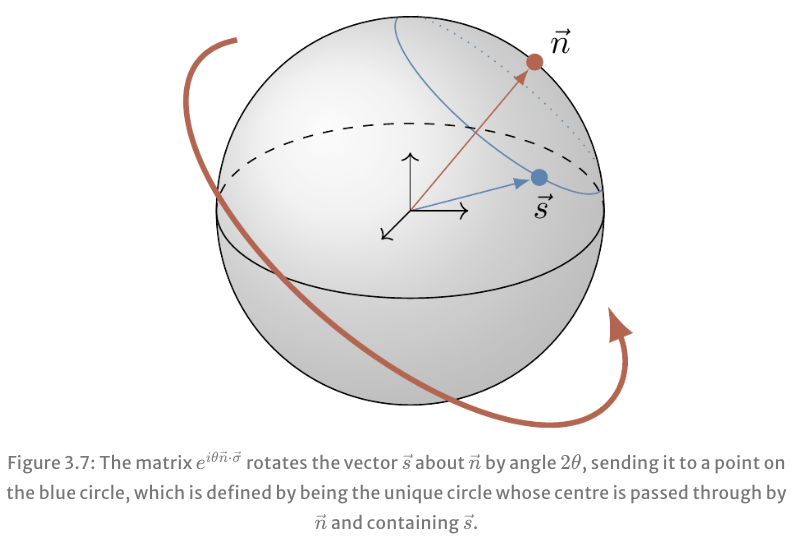
\includegraphics[width = 25em]{images/6.jpg}
\end{center}
\end{remark}

\begin{remark}[]
Though $U = e^{i\theta \vec{n}\cdot \vec{\sigma}}$ is typical, a better convention is $U = e^{-i\frac{\theta}{2} \vec{n}\cdot \vec{\sigma}}$ (equivalent up to global phase factor), because
\begin{itemize}
    \item The rotation is actually by $2\cdot \frac{\theta}{2} = \theta$.
    \item The direction of rotation follows right-hand rule in the Bloch sphere which is conventional in physics.
\end{itemize}
\end{remark}

\begin{example}[Pauli Rotations]
Now we can revisit the Pauli basis matrices in the form discussed in proposition \ref{prop:su2-decomposition-of-u} (they are so important that these rotations are called the Pauli rotations):
\begin{itemize}
    \item $e^{i\theta \sigma_x} = \cos\theta\mathbb{1} + (i\sin\theta)  \sigma_x = \begin{bmatrix}
        \cos\theta & i\sin\theta \\
        i\sin\theta & \cos\theta
    \end{bmatrix}$: \hl{$2\theta$-rotation about $x$-axis}.
    \item $e^{i\theta \sigma_y} = \cos\theta\mathbb{1} + (i\sin\theta)\sigma_y = \begin{bmatrix}
        \cos\theta & \sin\theta \\
        -\sin\theta & \cos\theta
    \end{bmatrix}$: \hl{$2\theta$-rotation about $y$-axis}.
    \item $e^{i\theta \sigma_z} = \cos(\theta)\mathbb{1} + (i\sin\theta)\sigma_z = \begin{bmatrix}
        \cos\theta + i\sin\theta & 0 \\
        0 & \cos\theta - i\sin\theta
    \end{bmatrix} = \begin{bmatrix}
        e^{i\theta} & 0 \\
        0 & e^{-i\theta}
    \end{bmatrix}$: \hl{$2\theta$-rotation about $z$-axis}.
\end{itemize}
\end{example}

\begin{example}[Hadamard Gate]
Recall $$
\begin{aligned}
H 
    &= \frac{1}{\sqrt{2}}\begin{bmatrix}
    1 & 1\\
    1 & -1
    \end{bmatrix} = \frac{1}{\sqrt{2}} (\sigma_x + \sigma_z)\\
    &= (-i)\left[(i\cdot 1)\frac{1}{\sqrt{2}} (\sigma_x + \sigma_z)\right]\\
    &= (-i)\left[ \prt{i\sin\frac{\pi}{2}}\vec{n}\cdot \vec{\sigma} \right]\\
    &= (-i) e^{i\frac{\pi}{2}\frac{1}{\sqrt{2}}(\sigma_x + \sigma_z)}
\end{aligned}
$$, which is exactly rotation by $\pi$ about the diagonal axis of the $x$-$z$-plane.
\end{example}


\subsection{$U\in U(2)$ acting on $V\in \RR^3$}
\begin{remark}
We can study the connection between unitaries and rotations by looking at how the unitary group $U(2)$ acts on the three-dimensional vector space of $2\times 2$ Hermitian matrices with zero trace (because all such matrices are simply $S = \vec{s} \cdot \vec{\sigma}$, so each $S$ can be represented by some $\vec{s}\in \RR^3$. Particularly, the first constant term is $0$ in the form we derived above).
\end{remark}

\begin{definition}[How does $U\in U(2)$ act on $V\in \RR^3$?]\label{defn:R_U}
It is defined by $$
R_U: \underset{S\subseteq}{\underbrace{\RR^3}}\rightarrow \underset{S'\subseteq}{\underbrace{\RR^3}}; R_U(s) = \vec{s'}\cdot \vec{\sigma} = U(\vec{s}\cdot \vec{\sigma})U^\dag
$$    
\end{definition}

\begin{definition}[isometry]
A map is an isometry if it preserves distance.
\end{definition}

\begin{proposition}[$R_U$ is an isometry]\label{prop:R_U-isometry}
Because $R_U$ preserves scalar product in the Euclidean space. Given $\vec{s}, \vec{t}$ as two arbitrary vectors:$$
\begin{aligned}
\vec{s'}\cdot \vec{t'}
    &\boxed{= \frac{1}{2}\Trace{S'T'}}\\
    &= \frac{1}{2}\Trace{\prt{USU^\dag}\prt{UTU^\dag}}\\
    &= \frac{1}{2}\Trace{\prt{U^\dag US}\prt{U^\dag UT}}\text{, cyclic property of $\Trace{\cdot}$}\\
    &= \frac{1}{2}\Trace{\prt{1\cdot S}\prt{1\cdot T}}\text{, $U$ is unitary}\\
    &\boxed{= \frac{1}{2}\Trace{ST}} = \vec{s} \cdot \vec{t}
\end{aligned}
$$
\end{proposition}

\begin{definition}[Orthogonal Transformation]
A linear transformation $T:V\rightarrow V$ on a inner product space $V$ is said to be orthogonal if the map preserves inner product (for example, in our particular case, it means dot product).
\end{definition}

\begin{proposition}[$R_U$ is an orthogonal map]
Clearly, by the justification of proposition \ref{prop:R_U-isometry}, we also know that $R_U$ is an orthogonal map.
\end{proposition}

\begin{theorem}[$R_U$ must be a rotation]\label{thm:R_U-is-rotation}
\end{theorem}
\begin{proof}
By proposition \ref{prop:R_U-isometry} we know that $R_U$ is an isometries. Furthermore, $\det{R_U} = 1$. It can be shown that the only isometries in $3$-dimentional Euclidean space described by orthogonal matrices with determinant $1$ are rotations (this part is hand-waved in the notes). So, $R_U$ must be a rotation.
\end{proof}

\begin{theorem}
Up to theorem \ref{thm:R_U-is-rotation}, we have shown a group homomorphism. Particularly, one such that $$
\underset{U\mapsto R_U}{U(2) \rightarrow SO(3)}
$$, where $SO$ means the \textbf{special orthogonal group} in three dimensions - the group of all rotations about the origin of $3$-dimensional Euclidean space $\RR^3$ under the operation of composition (which can be represented by the group of $3\times 3$ orthogonal (thus real) matrices.).
\end{theorem}

\begin{remark}
Referring back to what we have defined in definition \ref{defn:R_U}: $$
R_U(s) = U\prt{\vec{s}\cdot \vec{\sigma}}U^\dag
$$, we can see why we have been able to ignore the global phase factor: they will simply be cancelled out to $1$ under the above operation and come to represent the same rotation in $SO(3)$.
\end{remark}

\begin{remark}
The above mathematical argument secretly uses \textbf{quaternions}, a.k.a. \textbf{versors}, as they provide a very convenient way of describing spatial rotations (which are often used in $\eg$ $3D$ computer graphics).
\end{remark}

\subsection{Physics Interpretation}
Instead of the formal group object as described above, approximations for infinitesimal rotations are used in physics. Consider $\vec{s}\mapsto \vec{s'}$ induced by $$
U = e^{i\alpha \vec{n}\cdot\vec{\sigma}}
$$. So, for very small $\alpha$, we can do the following first order approximation of the Taylor expansion: $$
\begin{aligned}
\vec{s'} \cdot \vec{\sigma}
    &= U\prt{\vec{s}\cdot \vec{\sigma}} U^\dag\\
    &= e^{i\alpha \vec{n}\cdot \vec{\sigma}}\prt{\vec{s}\cdot \vec{\sigma}} e^{-i\alpha \vec{n}\cdot \vec{\sigma}}\\
    &= \prt{\Sum{i}{0}{\infty}\frac{(i\alpha \vec{n}\cdot \vec{\sigma})^n}{n!}}\prt{\vec{s}\cdot \vec{\sigma}} \prt{\Sum{i}{0}{\infty}\frac{(-i\alpha \vec{n}\cdot \vec{\sigma})^n}{n!}}\\
    &\approx \prt{1 + i\alpha \vec{n}\cdot \vec{\sigma}}\prt{\vec{s}\cdot \vec{\sigma}} \prt{1 - i\alpha \vec{n}\cdot \vec{\sigma}}\\
    &= \prt{\vec{s} + 2\alpha \vec{n}\times \vec{s}}\cdot \vec{\sigma}\\
\implies \boxed{\vec{s'}}
    &\boxed{= \vec{s} + 2\alpha \vec{n}\times \vec{s}}
\end{aligned}
$$. This is how usually how \hl{infinitesimal clockwise rotation of $\vec{s}$ about the $\vec{n}$-axis by an angle of $2\alpha$ is described in physics}.

\section{Universality (Revisited)}
Recall the universal set of gates that we discussed last week: any rotation in the Euclidean space can be performed as the following gate:
\begin{center}
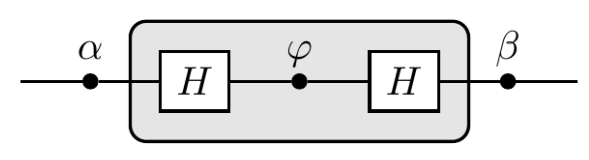
\includegraphics[width = 20em]{images/7.jpg}
\end{center}
That is, a rotation about $z$-axis, then a rotation about $x$-axis, followed by a final rotation about the $z$-axis. Based on these phase shifts and what we have just discussed in the last section, we can write this universal circuit as $$
\boxed{U(\alpha, \beta, \varphi) = e^{-i\frac{\beta}{2}\sigma_z}e^{-i\frac{\varphi}{2}\sigma_x}e^{-i\frac{\alpha}{2}\sigma_z}}
$$
Notice that: \begin{itemize}
    \item the phase shifts are taken to be counter-clockwise.
    \item angles in the formula are taken to be half of the angles actually rotated.
    \item the rotations applied are multiplied in order from right to left.
\end{itemize}

Next, we can write $U(\alpha, \beta, \varphi)$ as a matrix as well: $$
U(\alpha, \beta, \varphi) = e^{-i\frac{\beta}{2}\sigma_z}e^{-i\frac{\varphi}{2}\sigma_x}e^{-i\frac{\alpha}{2}\sigma_z} = \begin{bmatrix}
    e^{-i\prt{\frac{\alpha + \beta}{2}}}\cos\frac{\varphi}{2} & ie^{i\prt{\frac{\alpha - \beta}{2}}}\sin\frac{\varphi}{2} \\
    ie^{-i\prt{\frac{\alpha - \beta}{2}}}\sin\frac{\varphi}{2} & e^{-i\prt{\frac{\alpha + \beta}{2}}}\cos\frac{\varphi}{2}
    \end{bmatrix}
$$

\begin{remark}
Phase shift rotates a vector in a unit circle. With just the universal circuit as described above, it is possible to apply a limited number of phase gates (i.e. a set of $3$ phase shift gates) repeatedly, and reach within $\epsilon$ away from the intended point on the unit circle. However, this takes $$
\boxed{O\prt{\frac{1}{\epsilon}}}
$$ time.
\end{remark}

\begin{theorem}[Solovay-Kitaev]
Solovay-Kitaev showed that, if we compose $HTHT$ and $THTH$ gates instead of the classic universal circuit above (recall that $$
T = \begin{bmatrix}
1 & 0\\
0 & e^{i\frac{\pi}{4}}
\end{bmatrix}
$$). [The intuition why this works is that $THTH$ and $HTHT$ are not commutative operations (unlike the universal circuit), so it will have a lot more varieties once they are chained up.]

As it turns out, shown by Solovay and Kitaev through a constructive proof, that the time complexity for this gate to achieve $\epsilon$-approximation is only $$
\boxed{O\prt{\log\prt{\frac{1}{\epsilon}}}}
$$
\end{theorem}

\section{Quantum Dynamics}
\subsection{Time Evolution of a Quantum State}
The time evolution of a quantum state is a unitary process which is generated by a \underline{Hermitian operator} called the \textbf{Hamiltonian}, which we denote by $\hat{H}$.

\begin{proposition}
The Hamiltonian contains a complete specification of all interactions within the system under consideration - so, in general, the Hamiltonian changes over time.

Particularly, in an isolated system, the state vector $\Ket{\psi(t)}$ changes smoothly in time according to the Schrödinger equation: $$
\frac{d}{dt}\Ket{\psi(t)} = - \frac{i}{\hbar}\hat{H}\Ket{\psi(t)}
$$
\end{proposition}

\subsection{Newtonian $\rightarrow$ Lagrangian $\&$ Hamiltonian}
\begin{definition}
Newton describes how a mass changes over time in terms of forces and momentum. Specifically, $$
\vec{F} = \frac{d\vec{P}}{dt}
$$

Analogously, we don't have to describe a system by forces, but position (and so velocity, which is just the time derivative of position) instead, because $\vec{P} = m\vec{v}$ factors in $\vec{v}$ as part of it. Particularly, we can describe things entirely in terms of position, $q$:
\begin{itemize}
    \item in coordinates of $(\vec{q}, \dot{\vec{q}})$ (Lagrangian): we have the function $$
    \LLL(t, \vec{q}(t), \dot{\vec{q}}(t))
    $$ (defined by considering the difference of kinetic and potential energies). In this, we study the Euler-Langrange equations: $$
    \frac{d}{dt}\prt{\frac{\partial \LLL}{\partial \dot{\vec{q}}}} = \frac{\partial \LLL}{\partial \vec{q}}
    $$
    \item in coordinates of $(\vec{q}, \vec{p})$ (Hamiltonian): we have the function $$
    \HHH(t, \vec{q}(t), \vec{p}(t))
    $$ (defined by considering the sum of kinetic and potential energies). In this, we study the Hamiltonian equations: $$
    \begin{aligned}
        \frac{d\vec{q}}{dt} &= \frac{\partial \HHH}{\partial \vec{p}}\\
        \frac{d\vec{p}}{dt} &= \frac{\partial \HHH}{\partial \vec{q}}
    \end{aligned}
    $$
\end{itemize}
\end{definition}

\begin{remark}
In quantum, since momentum is a conserved quantity, whereas velocity is not, the Hamiltonian approach appears to be more useful than the others. The Hamiltonian approach is hidden in many things, like the position and momentum operators in quantum physics, uncertainty principles, etc.
\end{remark}

\begin{proposition}
For time-dependent Hamiltonian $\hat{H}(t)$, the formal solution of the Schrödinger equation is: $$
\Ket{\psi(t)} = e^{-\frac{i}{\hbar}\hat{H}t}\Ket{\psi(0)}
$$, which is clearly \textbf{separable}, as the LHS is just a product of two functions, where
\begin{itemize}
    \item The first function, with which we write $$
    U(t) = e^{-\frac{i}{\hbar}\hat{H}t}
    $$ is just a phase factor, which we have shown and believed to not affect the resulting probability.
    \item the second function has no time dependence.
\end{itemize}
So, $$
P = |\Ket{\psi(t)}|^2 = |U(t)|^2|\Ket{\psi(0)}|^2 = |\Ket{\psi(0)}|^2
$$, which means that \hl{$|\Ket{\psi(t)}|^2$ is constant over time}! We call such a state \textbf{stationary}, or a \textbf{standing wave}.
\end{proposition}


\end{document}